\let\negmedspace\undefined
\let\negthickspace\undefined
\documentclass[journal,12pt,onecolumn]{IEEEtran}
\usepackage{cite}
\usepackage{amsmath,amssymb,amsfonts,amsthm}
\usepackage{algorithmic}
\usepackage{graphicx}
\usepackage{textcomp}
\usepackage{xcolor}
\usepackage{txfonts}
\usepackage{listings}
\usepackage{enumitem}
\usepackage{mathtools}
\usepackage{gensymb}

\usepackage{tkz-euclide} % loads  TikZ and tkz-base
\usepackage{listings}



\newtheorem{theorem}{Theorem}[section]
\newtheorem{problem}{Problem}
\newtheorem{proposition}{Proposition}[section]
\newtheorem{lemma}{Lemma}[section]
\newtheorem{corollary}[theorem]{Corollary}
\newtheorem{example}{Example}[section]
\newtheorem{definition}[problem]{Definition}
%\newtheorem{thm}{Theorem}[section] 
%\newtheorem{defn}[thm]{Definition}
%\newtheorem{algorithm}{Algorithm}[section]
%\newtheorem{cor}{Corollary}
\newcommand{\BEQA}{\begin{eqnarray}}
\newcommand{\EEQA}{\end{eqnarray}}
\newcommand{\system}[1]{\stackrel{#1}{\rightarrow}}

\newcommand{\define}{\stackrel{\triangle}{=}}
\theoremstyle{remark}
\newtheorem{rem}{Remark}
%\bibliographystyle{ieeetr}
\begin{document}
%
\providecommand{\pr}[1]{\ensuremath{\Pr\left(#1\right)}}
\providecommand{\prt}[2]{\ensuremath{p_{#1}^{\left(#2\right)} }}        % own macro for this question
\providecommand{\qfunc}[1]{\ensuremath{Q\left(#1\right)}}
\providecommand{\sbrak}[1]{\ensuremath{{}\left[#1\right]}}
\providecommand{\lsbrak}[1]{\ensuremath{{}\left[#1\right.}}
\providecommand{\rsbrak}[1]{\ensuremath{{}\left.#1\right]}}
\providecommand{\brak}[1]{\ensuremath{\left(#1\right)}}
\providecommand{\lbrak}[1]{\ensuremath{\left(#1\right.}}
\providecommand{\rbrak}[1]{\ensuremath{\left.#1\right)}}
\providecommand{\cbrak}[1]{\ensuremath{\left\{#1\right\}}}
\providecommand{\lcbrak}[1]{\ensuremath{\left\{#1\right.}}
\providecommand{\rcbrak}[1]{\ensuremath{\left.#1\right\}}}
\newcommand{\sgn}{\mathop{\mathrm{sgn}}}
\providecommand{\abs}[1]{\left\vert#1\right\vert}
\providecommand{\res}[1]{\Res\displaylimits_{#1}} 
\providecommand{\norm}[1]{\left\lVert#1\right\rVert}
%\providecommand{\norm}[1]{\lVert#1\rVert}
\providecommand{\mtx}[1]{\mathbf{#1}}
\providecommand{\mean}[1]{E\left[ #1 \right]}
\providecommand{\cond}[2]{#1\middle|#2}
\providecommand{\fourier}{\overset{\mathcal{F}}{ \rightleftharpoons}}
\newenvironment{amatrix}[1]{%
  \left(\begin{array}{@{}*{#1}{c}|c@{}}
}{%
  \end{array}\right)
}
%\providecommand{\hilbert}{\overset{\mathcal{H}}{ \rightleftharpoons}}
%\providecommand{\system}{\overset{\mathcal{H}}{ \longleftrightarrow}}
    %\newcommand{\solution}[2]{\textbf{Solution:}{#1}}
\newcommand{\solution}{\noindent \textbf{Solution: }}
\newcommand{\cosec}{\,\text{cosec}\,}
\providecommand{\dec}[2]{\ensuremath{\overset{#1}{\underset{#2}{\gtrless}}}}
\newcommand{\myvec}[1]{\ensuremath{\begin{pmatrix}#1\end{pmatrix}}}
\newcommand{\mydet}[1]{\ensuremath{\begin{vmatrix}#1\end{vmatrix}}}
\newcommand{\myaugvec}[2]{\ensuremath{\begin{amatrix}{#1}#2\end{amatrix}}}
\providecommand{\rank}{\text{rank}}
\providecommand{\pr}[1]{\ensuremath{\Pr\left(#1\right)}}
\providecommand{\qfunc}[1]{\ensuremath{Q\left(#1\right)}}
    \newcommand*{\permcomb}[4][0mu]{{{}^{#3}\mkern#1#2_{#4}}}
\newcommand*{\perm}[1][-3mu]{\permcomb[#1]{P}}
\newcommand*{\comb}[1][-1mu]{\permcomb[#1]{C}}
\providecommand{\qfunc}[1]{\ensuremath{Q\left(#1\right)}}
\providecommand{\gauss}[2]{\mathcal{N}\ensuremath{\left(#1,#2\right)}}
\providecommand{\diff}[2]{\ensuremath{\frac{d{#1}}{d{#2}}}}
\providecommand{\myceil}[1]{\left \lceil #1 \right \rceil }
\newcommand\figref{Fig.~\ref}
\newcommand\tabref{Table~\ref}
\newcommand{\sinc}{\,\text{sinc}\,}
\newcommand{\rect}{\,\text{rect}\,}
%%
%   %\newcommand{\solution}[2]{\textbf{Solution:}{#1}}
%\newcommand{\solution}{\noindent \textbf{Solution: }}
%\newcommand{\cosec}{\,\text{cosec}\,}
%\numberwithin{equation}{section}
%\numberwithin{equation}{subsection}
%\numberwithin{problem}{section}
%\numberwithin{definition}{section}
%\makeatletter
%\@addtoreset{figure}{problem}
%\makeatother

%\let\StandardTheFigure\thefigure
\let\vec\mathbf


\bibliographystyle{IEEEtran}
\title{Gate 2023 EC 58}
\author{HIBA MUHAMMED\\
        EE23BTECH11026}
\maketitle

\section*{Problem Statement}
Let $x_1(t) = u(t + 1.5) - u(t - 1.5)$ and $x_2(t)$ is shown in the figure below. For $y(t) = x_1(t) * x_2(t)$, the $\int_{-\infty}^{\infty} y(t) \, dt$ is \underline{\hspace{2cm}}.

\begin{figure}[htbp]
    \centering
    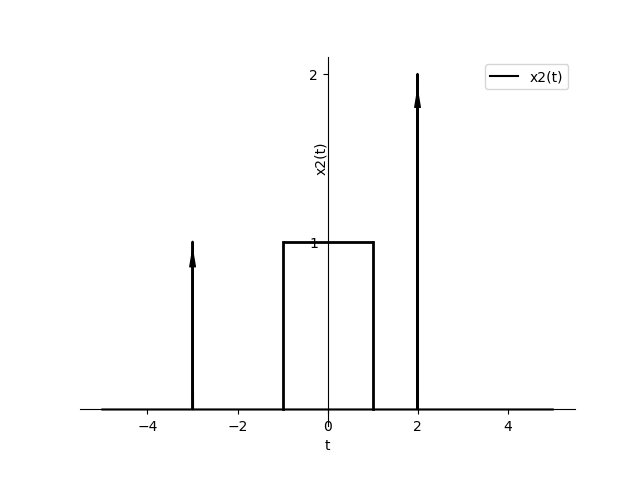
\includegraphics[width=0.5\textwidth]{gatefig.png}
    \caption{Figure}
    \label{fig:graph}
\end{figure}

\section*{Solution}
\section*{Input Parameters}
\begin{table}[htbp]
    \centering
    \begin{tabular}{|c|c|p{6cm}|}
        \hline
        \multicolumn{3}{|c|}{\textbf{Input Parameters}} \\
        \hline
        \textbf{Function} & \textbf{Expression} & \textbf{Description} \\
        \hline
        $x_1(t)$ & $u(t + 1.5) - u(t - 1.5)$ & Step function with delay and width parameters. \\
        \hline
        $X_1(f)$ &  & Fourier Transform of $x_1(t)$. \\
        \hline
        $x_2(t)$ & $\delta(t + 3) + \text{rect}\left(\frac{t}{2}\right) + 2\delta(t - 2)$ & Impulse function followed by a rectangle and two impulses. \\
        \hline
        $X_2(f)$ &  & Fourier Transform of $x_2(t)$. \\
        \hline
    \end{tabular}
\end{table}

\begin{align}
x_1(t) &= u(t+1.5) - u(t-1.5) \\
x_1(t) &= \text{rect}\left(\frac{t}{3}\right) \\
\end{align}


The Fourier Transform of $rect\left(\frac{t}{a}\right)$:

\begin{align}
\text{rect}\left(\frac{t}{a}\right) &\xleftrightarrow{\mathcal{F}} a \times \sin(2\pi f \frac{a}{2}) \\
\text{where } \text{rect}\left(\frac{t}{a}\right) &= \begin{cases}
1 & \text{if } |t| < \frac{a}{2} \\
0 & \text{otherwise}
\end{cases}\\
& X_1(f)=3\text{sinc}(1.5\cdot 2\pi f) & \\
& x_2(t) = \delta(t+3) + \text{rect}\left(\frac{t}{2}\right) + 2\delta(t-2) & \\
& X_2(f) = e^{3j\cdot 2\pi f} + 2\text{sinc}(2\pi f) + 2e^{-2j \cdot 2\pi f} & \\
& y(t) = x_1(t) * x_2(t) \\
& \text taking \hspace{0.2cm}inverse \\
& y(t) = \text{rect}\left(\frac{t+3}{3}\right) + 2\text{rect}\left(\frac{t-2}{3}\right) + (t+2.5)u(t+2.5) + (t-2.5)u(t-2.5) \\
& - (t+0.5)u(t+0.5) - (t-0.5)u(t-0.5)\\
& Y(f) = X_1(f) \cdot X_2(f) \\
&\hspace{1cm}= 3\text{sinc}(1.5 \cdot 2\pi f) \cdot (e^{3j \cdot 2\pi f} + 2\text{sinc}(2\pi f) + 2e^{-2j \cdot 2\pi f})\\
& Y(0)= 3\text{sinc}(0) \cdot (e^{0} + 2\text{sinc}(0) + 2e^{0}) \\
&\hspace{1cm}= 3\cdot (1 + 2 + 2) \\
&\hspace{1cm}= 15
\end{align}



Therefore, the value of $\int_{-\infty}^{\infty} y(t) \, dt$ is $15$


\begin{figure}[htbp]
    \centering
    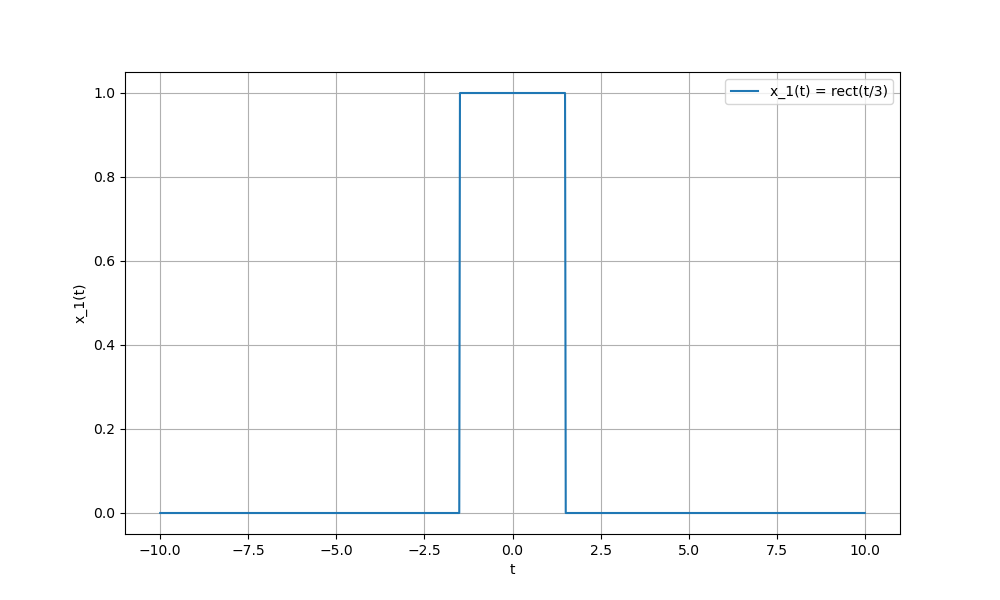
\includegraphics[width=0.8\textwidth]{gate_x1.png}
    \caption{Graph of \(x_1(t) = \text{rect}\left(\frac{t}{3}\right)\)}
    \label{fig:x_1_graph}
\end{figure}


\begin{figure}[htbp]
    \centering
    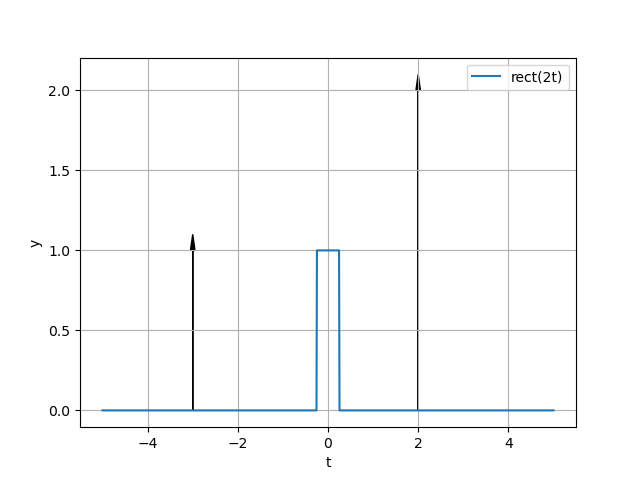
\includegraphics[width=0.8\textwidth]{gate_x2.png}
    \caption{Graph of \(x_2(t) = \delta(t+3) + \text{rect}(2t) + 2\delta(t-2)\)}
    \label{fig:x_2_graph}
\end{figure}


\begin{figure}[htbp]
    \centering
    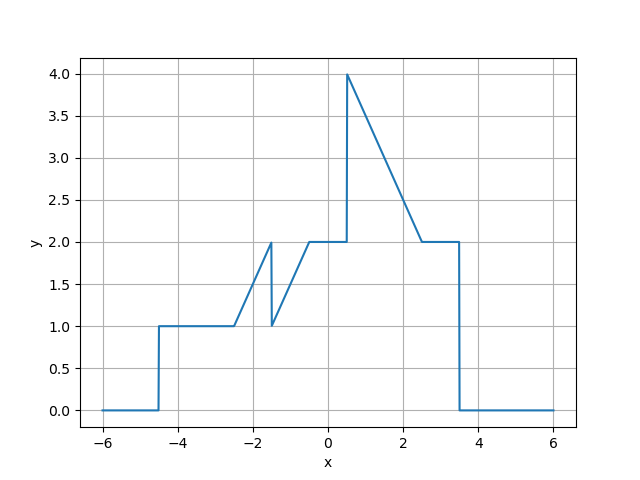
\includegraphics[width=0.8\textwidth]{gate_y.png}
    \caption{Graph of \(y(t)\)}
    \label{fig:x_2_graph}
\end{figure}
\end{document}
